\documentclass{article}
\usepackage{amsmath,accents}%
\usepackage{amsfonts}%
\usepackage{amssymb}%
\usepackage{comment}
\usepackage{graphicx}
\usepackage{mathrsfs}
\usepackage[utf8]{inputenc}
\usepackage{amsfonts}
\usepackage{amssymb}
\usepackage{graphicx}
\usepackage{mathrsfs}
\usepackage{setspace}
\usepackage{amsthm}
\usepackage{nccmath}
\usepackage[spanish]{babel}
\usepackage{multirow}
\usepackage{hyperref}
\usepackage{tikz-cd}
\usepackage{pgf,tikz}
\usetikzlibrary{arrows}
\usetikzlibrary{cd}
\usetikzlibrary{babel}
\theoremstyle{plain}

\renewcommand{\baselinestretch}{1,4}
\setlength{\oddsidemargin}{0.5in}
\setlength{\evensidemargin}{0.5in}
\setlength{\textwidth}{5.4in}
\setlength{\topmargin}{-0.25in}
\setlength{\headheight}{0.5in}
\setlength{\headsep}{0.6in}
\setlength{\textheight}{8in}
\setlength{\footskip}{0.75in}

\theoremstyle{definition}

\newtheorem{theorem}{Teorema}[section]
\newtheorem{acknowledgement}{Acknowledgement}
\newtheorem{algorithm}{Algorithm}
\newtheorem{axiom}{Axiom}
\newtheorem{case}{Case}
\newtheorem{claim}{Claim}
\newtheorem{propi}[theorem]{Propiedades}
\newtheorem{condition}{Condition}
\newtheorem{conjecture}{Conjecture}
\newtheorem{coro}[theorem]{Corolario}
\newtheorem{criterion}{Criterion}
\newtheorem{defi}[theorem]{Definición}
\newtheorem{example}[theorem]{Ejemplo}
\newtheorem{exercise}{Ejercicio}
\newtheorem{lemma}[theorem]{Lema}
\newtheorem{nota}[theorem]{Nota}
\newtheorem{sol}{Solución}
\newtheorem*{sol*}{Solución}
\newtheorem{prop}[theorem]{Proposición}
\newtheorem{remark}{Remark}

\newtheorem{dem}[theorem]{Demostración}

\newtheorem{summary}{Summary}

\providecommand{\abs}[1]{\lvert#1\rvert}
\providecommand{\norm}[1]{\lVert#1\rVert}
\providecommand{\ninf}[1]{\norm{#1}_\infty}
\providecommand{\numn}[1]{\norm{#1}_1}
\providecommand{\gabs}[1]{\left|{#1}\right|}
\newcommand{\bor}[1]{\mathcal{B}(#1)}
\newcommand{\R}{\mathbb{R}}
\newcommand{\Q}{\mathbb{Q}}
\newcommand{\Z}{\mathbb{Z}}
\newcommand{\F}{\mathbb{F}}
\newcommand{\X}{\chi}
\providecommand{\Zn}[1]{\Z / \Z #1}
\newcommand{\resi}{\varepsilon_L}
\newcommand{\cee}{\mathbb{C}}
\providecommand{\conv}[1]{\overset{#1}{\longrightarrow}}
\providecommand{\gene}[1]{\langle{#1}\rangle}
\providecommand{\convcs}{\xrightarrow{CS}}
% xrightarrow{d}[d]
\setcounter{exercise}{0}
\newcommand{\cicl}{\mathcal{C}}

\newenvironment{ejercicio}[2][Estado]{\begin{trivlist}
\item[\hskip \labelsep {\bfseries Ejercicio}\hskip \labelsep {\bfseries #2.}]}{\end{trivlist}}
%--------------------------------------------------------
\begin{document}
\title{Relación 3 - Geometría y Topología de superficies }
\author{Javi, Rafa, Diego}
\maketitle
\begin{exercise}
Probar que si $f:X\to S^n$ no es epiyectiva entonces es homotópica a la aplicación constante.
\end{exercise}
\begin{sol*}
Sea $y\in S^n\setminus f(X)$. Mediante la proyección estereográfica existe un homeomorfismo $p:S^n\setminus\{y\}\to\R^n$, por lo que se induce una aplicación continua $p\circ f:X\to\R^n$. Como $\R^n$ es contráctil, $p\circ f\simeq x_0\in\R^n$. Como $p$ es homeomorfismo, tiene una inversa continua $p^{-1}$, y componiendo obtenemos $p^{-1}\circ p\circ f= f\simeq p^{-1}(x_0)$. Por lo que $f$ es nul-homotópica. 
\end{sol*}
\newpage
\begin{exercise}
Probar que todo retracto de un espacio métrico es un subespacio cerrado.
\end{exercise}
\begin{sol*}
Sea $X$ un espacio métrico y $A\subseteq X$ un retracto. Por hipótesis existe una aplicación continua $r:X\to A$ tal que $r(a)=a\ \forall a\in A$. Sea $\{x_n\}\subset A$ una sucesión que converge a un punto $x\in X$. Tenemos que probar que $x\in A$. Tenemos que $r(x_n)$ converge a $r(x)$. Además, $r(x_n)=x_n\ \forall n$ por ser una sucesión de $A$. Por lo tanto, al tratarse de un espacio métrico (y por tanto Hausdorff) $r(x)=x$, y como $r(x)\in A$ por definición, se tiene el resultado. 
\end{sol*}
\newpage
\begin{exercise}
Probar que $A$ es retracto de $X$ si y sólo si toda función continua de $A$ es un espacio arbitrario $Z$ admite una extensión continua sobre $X$.
\end{exercise}
\begin{sol*}
$\boxed{\Rightarrow}$ Supongamos que $A$ es retracto de $X$. Sea $f:A\to Z$ una función continua y sea $r:X\to A$ una retracción. Entonces la extensión continua sobre $X$ es $r\circ f$. Efectivamente es continua por ser composición de continuas.\\
$\boxed{\Leftarrow}$ Para el recíproco, sea $Z=A$ y sea $f=Id_A$. Entonces la extensión continua sobre $X$ es una retracción. Efectivamente, si $g$ es dicha extensión, entonces $g:X\to A$ y como $g(a)=Id_A(a)=a\ \forall a\in A$, se tiene el resultado. 
\end{sol*}
\newpage
\begin{exercise}
Probar que si $A$ y $B$ son retractos de deformación de $X$ e $Y$ respectivamente, entonces $A\times B$ es retracto de deformación de $X\times Y$.
\end{exercise}
\begin{sol*}
Por hipótesis existen $r_1:X\to A$ y $r_2:Y\to B$ continuas tales que $r_1(a)=a\ \forall a\in A$ y $r_2(b)=b\ \forall b\in B$. Podemos construir entonces la aplicación $r:X\times Y\to A\times B$ definida como $r(x,y)=(r_1(x),r_2(y))$ que cumple claramente $r(a,b)=(a,b)\ \forall (a,b)\in A\times B$ y además es continua por ser el producto de aplicaciones continuas. Hasta ahora hemos probado que $A\times B$ es retraco de $X\times Y$, ahora tenemos que probar que es de deformación. Por hipótesis $i_1\circ r_1\simeq Id_X$ e $i_2\circ r_2\simeq Id_Y$, donde $i_1$ e $i_2$ son las respectivas inclusiones. Sean $H_1$ y $H_2$ las homotopías correspondientes. Vamos a construir una homotopía entre $i\circ r$ y $Id_{X\times Y}$, donde $i=i_1\times i_2$. Basta tomar $H:X\times Y\times I\to X\times Y$ definida como $H((x,y),t)=H_1(x,t)\times H_2(y,t)$, que es continua por ser producto de continuas y cumple por hipótesis
\begin{gather*}
H((x,y),0)=H_1(x,0)\times H_2(y,0)= (x,y)\\
H((x,y),1)=H_1(x,1)\times H_2(y,0)= (i_1(r_1(x)),i_2(r_2(y)).
\end{gather*}
Esto finaliza el ejercicio.
\end{sol*}
\newpage
\begin{exercise}
Probar que si $A$ es retracto de deformación de $X$ y $B$ lo es de $A$, entonces $B$ lo es de $X$. 
\end{exercise}
\begin{sol*}
Por hipótesis existe una función continua $H:X\times I\to X$ que cumple $H(x,0)=x$, $H(x,1)\in A$, y $H(a,t)=a\ \forall a\in A$. También existe $G:A\times I\to A$ cumpliendo $G(a,0)=a$, $G(a,1)\in B$ y $G(b,t)=b\ \forall b\in B$. La idea será retraer con deformación $X$ hasta convertirlo en $A$ y luego continuar hasta convertirlo en $B$. Sea $F:X\times I\to X$ definida como sigue
\[
F(x,t)=\begin{cases}
H(x,2t) & t\in\left[0,\frac{1}{2}\right]\\
G(H(x,1),2t-1) & t\in\left[\frac{1}{2},1\right]
\end{cases},
\]
que es continua puesto que $F(\frac{1}{2},t)=G(H(x,1),0)=H(x,1)$. Comprobamos que se tiene
\begin{gather*}
F(x,0)=H(x,0)=x\\
F(x,1)=G(H(x,1),1)\in B\\
F(b,t)=H(b,t)=b\ \forall t\in \left[0,\frac{1}{2}\right]\ \forall b\in B\\
F(b,t)=G(H(b,1),2t-1)=H(b,1)=b\ \forall t\in\left[\frac{1}{2},1\right] \ \forall b\in B.
\end{gather*}
Con lo que ya hemos terminado. 
\end{sol*}
\newpage
\begin{exercise}Dar un ejemplo de un espacio $X$ y de dos subconjuntos $A$ y $B$ homeomorfos tales que $A$ sea retracto de deformación de $X$ y $B$ no lo sea.
\end{exercise}
\begin{sol*}
Sea $X=X_1\cup X_2$ un compacto de $\R^2$ formado por dos componentes conexas $X_1$ y $X_2$ tal como se ve en la figura más abajo. Sea $A=\{a_1,a_2\}$ con $a_1\in X_2$ y $a_2\in X_2$. Sea $B=\{b_1,b_2\}\subset X_1$. Como cada $X_i$ es contráctil, $X_1$ puede retraerse con deformación sobre $a_1$ y lo mismo con $X_2$ sobre $a_2$. Pero $B$ no puede ser retracto de deformación, ya que ambos puntos están en una misma componente conexa. Pero $A\cong B$, pues ambos son dos puntos. 
\definecolor{qqqqff}{rgb}{0.3333333333333333,0.3333333333333333,0.3333333333333333}
\definecolor{zzttqq}{rgb}{0.26666666666666666,0.26666666666666666,0.26666666666666666}
\begin{tikzpicture}[line cap=round,line join=round,>=triangle 45,x=1.0cm,y=1.0cm]
\clip(-8.293333333333335,-0.43333333333333324) rectangle (7.04,6.993333333333332);
\fill[color=zzttqq,fill=zzttqq,fill opacity=0.10000000149011612] (-5.,5.) -- (-2.,5.) -- (-2.,1.) -- (-5.,1.) -- cycle;
\fill[color=zzttqq,fill=zzttqq,fill opacity=0.10000000149011612] (-1.,5.) -- (-1.,1.) -- (2.,1.) -- (2.,5.) -- cycle;
\draw [color=zzttqq] (-5.,5.)-- (-2.,5.);
\draw [color=zzttqq] (-2.,5.)-- (-2.,1.);
\draw [color=zzttqq] (-2.,1.)-- (-5.,1.);
\draw [color=zzttqq] (-5.,1.)-- (-5.,5.);
\draw [color=zzttqq] (-1.,5.)-- (-1.,1.);
\draw [color=zzttqq] (-1.,1.)-- (2.,1.);
\draw [color=zzttqq] (2.,1.)-- (2.,5.);
\draw [color=zzttqq] (2.,5.)-- (-1.,5.);
\draw (-4,5.91) node[anchor=north west] {$\Large{X_1}$};
\draw (0.,5.91) node[anchor=north west] {$\Large{X_2}$};
\draw (-3.6,2.2) node[anchor=north west] {$\Large{a_1}$};
\draw (0.36,2.2) node[anchor=north west] {$\Large{a_2}$};
\draw (-3.6,4.2) node[anchor=north west] {$\Large{b_1}$};
\draw (-3.56,3.2) node[anchor=north west] {$\Large{b_2}$};
\begin{scriptsize}
\draw [fill=qqqqff] (-4.,4.) circle (2.5pt);
\draw [fill=qqqqff] (-4.,3.) circle (2.5pt);
\draw [fill=qqqqff] (-4.,2.) circle (2.5pt);
\draw [fill=qqqqff] (0.,2.) circle (2.5pt);
\end{scriptsize}
\end{tikzpicture}
\end{sol*}
\newpage
\begin{exercise}
Probar que $S^{n-1}$ es retracto de deformación de $R^n-\{0\}$. Encontrar retractos de deformación (compactos) de los siguientes espacios.
\begin{enumerate}
\item $\R^2-\{p_1,p_2,\dotsc,p_k\}$,
\item $S^1\times S^1-\{*\}$ (el toro menos un punto),
\item $\R^3-OZ$, $\R^3-S^1\lor S^1$,
\item la banda de Möbius y la banda de Möbius menos un punto,
\item $\R^4-(OZ\bigcup S^1)$,
\item el complementario de un disco en el plano proyectivo y
\item el complementario en $\R^3$ de dos rectas paralelas.
\end{enumerate}
\end{exercise}
\begin{sol*}
Sea $i$ la inclusión $i:S^{n-1}\hookrightarrow\R^n\setminus\{0\}$ y sea $r:\R^n\setminus\{0\}\to S^{n-1}$ dada por $r(x)=\frac{x}{\norm{x}}$. Tenemos que probar que $r\circ i\simeq Id_{S^{n-1}}$ y que $i\circ r\simeq Id_{\R^n\setminus\{0\}}$. La primera es trivial pues $r\circ i= Id_{S^{n-1}}$. Para la segunda definimos $H(x,t)=(1-t)x+t\frac{x}{\norm{x}}$ que cumple $H(x,0)=x=Id(x)$ y $H(x,1)=\frac{x}{\norm{x}}=i(r(x))$, la cual es claramente continua.
\begin{enumerate}
\item $\bigvee_{p_1}^{p_k}S^1$.
\item $S^1\vee S^1$.

\definecolor{ffffff}{rgb}{1.,1.,1.}
\begin{tikzpicture}[line cap=round,line join=round,>=triangle 45,x=1.0cm,y=1.0cm]
\clip(-2.0933333333333337,-1) rectangle (13.24,4);
\fill[fill=black,fill opacity=0.10000000149011612] (3.,3.) -- (0.,3.) -- (0.,0.) -- (3.,0.) -- cycle;
\draw [color=ffffff,fill=ffffff,fill opacity=1.0] (1.4933333333333336,1.4733333333333323) circle (0.44402202147591235cm);
\draw (3.,3.)-- (0.,3.);
\draw (0.,3.)-- (0.,0.);
\draw (0.,0.)-- (3.,0.);
\draw (3.,0.)-- (3.,3.);
\draw [->] (0.,3.) -- (1.6,3.);
\draw [->] (0.,0.) -- (1.5866666666666671,0.);
\draw [->] (0.,0.) -- (0.,1.66);
\draw [->] (3.,0.) -- (3.,1.54);
\draw [->,dash pattern=on 2pt off 2pt] (1.826666666666667,1.7666666666666655) -- (2.266666666666667,2.0733333333333324);
\draw [->,dash pattern=on 2pt off 2pt] (1.44145324639669,1.9143140722947996) -- (1.44,2.4066666666666654);
\draw [->,dash pattern=on 2pt off 2pt] (1.104009315179931,1.6868336013529408) -- (0.7466666666666668,2.0066666666666655);
\draw [->,dash pattern=on 2pt off 2pt] (1.0604746885923042,1.3743942145353825) -- (0.5066666666666668,1.4066666666666656);
\draw [->,dash pattern=on 2pt off 2pt] (1.5361033970521951,1.0313760082384311) -- (1.5333333333333337,0.5133333333333324);
\draw [->,dash pattern=on 2pt off 2pt] (1.2387034239488126,1.109576319926874) -- (1.,0.78);
\draw [->,dash pattern=on 2pt off 2pt] (1.9323447901837905,1.406816445931748) -- (2.4666666666666672,1.4066666666666656);
\draw [->,dash pattern=on 2pt off 2pt] (1.8251995298851869,1.178341158620574) -- (2.306666666666667,0.74);
\draw [->] (4.,1.46) -- (5.08,1.4466666666666657);
\draw (6.,3.)-- (6.,0.);
\draw (6.,0.)-- (9.,0.);
\draw (9.,0.)-- (9.,3.);
\draw (9.,3.)-- (6.,3.);
\draw [->] (6.,3.) -- (7.626666666666668,3.);
\draw [->] (9.,0.) -- (9.,1.5666666666666655);
\draw [->] (6.,0.) -- (6.,1.5133333333333323);
\draw [->] (6.,0.) -- (7.56,0.);
\draw (1.32,3.7) node[anchor=north west] {$\Large{A}$};
\draw (7.133333333333335,3.7266666666666652) node[anchor=north west] {$\Large{A}$};
\draw (1.186666666666667,0.03333333333333257) node[anchor=north west] {$\Large{A}$};
\draw (7.28,-0.02) node[anchor=north west] {$\Large{A}$};
\draw (-0.7466666666666668,1.86) node[anchor=north west] {$\Large{B}$};
\draw (3.2,1.8333333333333321) node[anchor=north west] {$\Large{B}$};
\draw (5.44,1.7) node[anchor=north west] {$\Large{B}$};
\draw (9.173333333333336,1.7933333333333321) node[anchor=north west] {$\Large{B}$};
\draw (4.386666666666668,1.98) node[anchor=north west] {$\Large{r}$};
\end{tikzpicture}  

\item $S^1$ (se retrae sobre $\R^2\setminus\{0\}$ con la proyección y luego a $S^1$). $S^2\vee T^2$ como se puede ver en la imagen. 
\begin{figure}[h!]
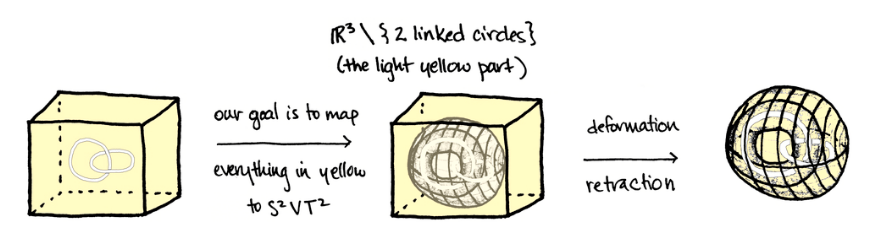
\includegraphics[scale=0.6]{S2wedgeT2}
\end{figure}  

\newpage

\item En el primer caso $S^1$. Vamos a definir la retracción sobre la Banda de Möbius vista como su polígono fundamental. Es decir $B=I\times I/\sim$ donde $(1,t)\sim (0,1-t)$. Sea pues $r:B\to S^1$ definida como $r([x,t])\mapsto [\frac{1}{2},t]$. Esta aplicación es claramente continua y cumple que $r\circ i_{S^1}=Id_{S^1}$. Tenemos que probar entonces que $i\circ r\simeq Id_{B}$. Sea $H:B\times I\to B$ definida como $H([x,t],s)=[\frac{1}{2}+(x-\frac{1}{2})s,t]$, Es fácil comprobar que cumple lo requerido. \\
En el segundo caso es $S^1\vee S^1$. Lo vemos gráficamente. 

\definecolor{ffffff}{rgb}{1.,1.,1.}
\begin{tikzpicture}[line cap=round,line join=round,>=triangle 45,x=1.0cm,y=1.0cm]
\clip(-2.0933333333333337,-1.) rectangle (13.026666666666669,4);
\fill[fill=black,fill opacity=0.10000000149011612] (3.,3.) -- (0.,3.) -- (0.,0.) -- (3.,0.) -- cycle;
\draw [color=ffffff,fill=ffffff,fill opacity=1.0] (1.4933333333333336,1.4733333333333323) circle (0.44402202147591235cm);
%\fill(6.,3.) -- (6.,0.) -- (9.,0.) -- (9.,3.) -- cycle;
\draw (3.,3.)-- (0.,3.);
\draw (0.,3.)-- (0.,0.);
\draw (0.,0.)-- (3.,0.);
\draw (3.,0.)-- (3.,3.);
\draw [->] (0.,3.) -- (1.6,3.);
\draw [->] (0.,0.) -- (1.5866666666666671,0.);
\draw [->,dash pattern=on 2pt off 2pt] (1.826666666666667,1.7666666666666655) -- (2.266666666666667,2.0733333333333324);
\draw [->,dash pattern=on 2pt off 2pt] (1.44145324639669,1.9143140722947996) -- (1.44,2.4066666666666654);
\draw [->,dash pattern=on 2pt off 2pt] (1.104009315179931,1.6868336013529408) -- (0.7466666666666668,2.0066666666666655);
\draw [->,dash pattern=on 2pt off 2pt] (1.0604746885923042,1.3743942145353825) -- (0.5066666666666668,1.4066666666666656);
\draw [->,dash pattern=on 2pt off 2pt] (1.5361033970521951,1.0313760082384311) -- (1.5333333333333337,0.5133333333333324);
\draw [->,dash pattern=on 2pt off 2pt] (1.2387034239488126,1.109576319926874) -- (1.,0.78);
\draw [->,dash pattern=on 2pt off 2pt] (1.9323447901837905,1.406816445931748) -- (2.4666666666666672,1.4066666666666656);
\draw [->,dash pattern=on 2pt off 2pt] (1.8251995298851869,1.178341158620574) -- (2.306666666666667,0.74);
\draw [->] (4.,1.46) -- (5.08,1.4466666666666657);
\draw (6.,3.)-- (6.,0.);
\draw (6.,0.)-- (9.,0.);
\draw (9.,0.)-- (9.,3.);
\draw (9.,3.)-- (6.,3.);
\draw [->] (6.,3.) -- (7.626666666666668,3.);
\draw [->] (6.,0.) -- (7.56,0.);
\draw (1.32,3.7) node[anchor=north west] {$\Large{A}$};
\draw (7.133333333333335,3.7266666666666652) node[anchor=north west] {$\Large{A}$};
\draw (1.186666666666667,0.03333333333333182) node[anchor=north west] {$\Large{A}$};
\draw (7.28,-0.02) node[anchor=north west] {$\Large{A}$};
\draw (4.386666666666668,1.98) node[anchor=north west] {$\Large{r}$};
\end{tikzpicture}

\item $T^2$. Partimos de
\begin{figure}[h!]
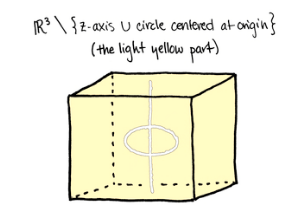
\includegraphics[scale=0.7]{T2-1}
\end{figure}\

En cada sección plana perpendicular al plano $XY$ hacemos lo siguiente
\begin{figure}[h!]
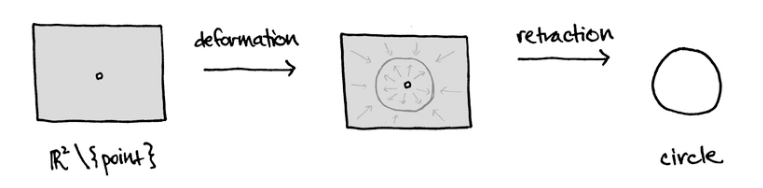
\includegraphics[scale=0.6]{T2-2}
\end{figure}

Visto en el espacio tendríamos lo siguiente
\begin{figure}[h!]
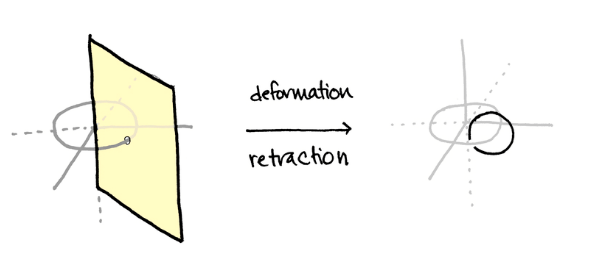
\includegraphics[scale=0.6]{T2-3}
\end{figure}

Finalmente rotamos entorno al eje $0Z$.

\begin{figure}[h!]
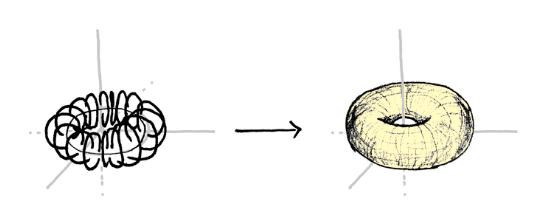
\includegraphics[scale=0.6]{T2-4}
\end{figure}

\item $S^1$. Podemos empujar el agujero hasta los bordes y luego pegar con las identificaciones, de modo que queda una circunferencia. La retracción, suponiendo que el agujero está en el centro, sería $r:\mathbb{P}_2\R\to S^1$ definida como $r(x)=\frac{x}{||x||}$. La homotopía para que $i\circ r\simeq Id$ es $H: \mathbb{P}_2\R\times I\to \mathbb{P}_2\R$ tal que $H(x,t)=(1-t)x+\frac{x}{||x||}t$. 
\item $S^1\vee S^1$. Ya que podemos considerar un semiespacio por cada recta, que sería homeomorfo al primero del apartado $3$. Luego basta unirlos por un punto. 
\end{enumerate}
\end{sol*}
\newpage
\begin{exercise}
Probar que si $X$ es contráctil e $Y$ arcoconexo, dos aplicaciones cualesquiera de $X$ en $Y$ son homotópicas.
\end{exercise}
\begin{sol*}
Por ser $X$ contráctil, $Id_X\simeq x_0$ mediante una homotopía $F:X\times I\to X$. Sea $f:X\to Y$ una aplicación continua y sea $f\circ F: X\times I\to Y$ la aplicación $(x,t)\mapsto f(F(x,t))$, que nos da una homotopía entre $f$ y la aplicación constante $f(x_0)$. Dado $y\in Y$ sea $\gamma: I\to Y$ un camino desde $f(x_0)$ hasta $y$. Definimos entonces la homotopía $G:X\times I\to Y$ como $G(x,t)=\gamma(t)$. Por lo tanto, dadas $f,g:X\to Y$ funciones continuas, podemos partir de $f(x_0)$ y llegar a $y=g(x_0)$ con la siguiente homotopía $H:X\times Y\to Y$,
$$
H(x,t)=\begin{cases}
f(F(x,t)) & t\in[0,\frac{1}{2}]\\
\gamma(t) & t\in[\frac{1}{2},1]
\end{cases},
$$
que claramente es continua.
\end{sol*}
\newpage
\begin{exercise}
Indicar cuántos elementos tiene el conjunto de las clases de homotopía de aplicaciones continuas de $(S^1,\{1\})$ en $(X,*)$ rel. $\{1\}$, en los casos siguientes:
\begin{enumerate}
\item $X$ tiene la topología discreta.
\item $X$ tiene la topología indiscreta.
\end{enumerate}

\end{exercise}
\begin{sol*}
\begin{enumerate}
\item[]
\item Si $X$ tiene la topología discreta, las únicas funciones continuas entre $S^1$ y $X$ son las constantes. Efectivamente, sea $x\in X$ y $z\in S^1$ tal que $f(z)=x$, para alguna función continua $f:S^1\to X$. Entonces $z\in f^{-1}(\{x\})$ y como por continuidad $f^{-1}(\{x\})$ es abierto, $z$ tiene un entorno donde la función es constante igual a $x$. Este razonamiento vale para todos los puntos de $S^1$, luego todos tienen un entorno constante. Como $S^1$ es conexa esta constante es la misma en todo los entornos, de lo contrario podríamos cubrir $S^1$ por abiertos disjuntos. Por lo tanto, hay tantas funciones continuas como elementos tiene $X$. Ahora bien, no hay ninguna homotopía entre dos funciones constantes que deje fijo un elemento, por lo tanto las clases de homotopía relativa a $\{1\}$ solo tienen un elemento y el conjunto de clases tiene el mismo cardinal que $X$. 
\item Si $X$ tiene la topología indiscreta entonces toda función de $S^1$ en $X$ es continua. Este hecho es claro porque los únicos abiertos son $X$ y $\emptyset$, por lo que o bien tenemos $f^{-1}(X)=S^1$ o bien $f^{-1}(\emptyset)=\emptyset$, que son abiertos. Este razonamiento vale para cualquier espacio de partida, en particular para el $[0,1]$, luego toda función $\gamma:[0,1]\to X$ es un camino. Es decir que dadas dos funciones $f,g:S^1\to X$ existe un camino $\gamma_x(t)$ entre $f(x)$ y $g(x)$. En el caso de $f(1)=g(1)$ sería el camino trivial de un solo punto. Por lo tanto podemos definir una homotopía $H:S^1\times I\to X$ que relacione cualesquiera dos funciones definiéndola como $H(x,t)=\gamma_x(t)$. Esta homotopía es continua de nuevo porque va a un espacio con topología indiscreta. En definitiva, solo existe una clase de homotopía en este caso.
\end{enumerate}
\end{sol*}
\newpage
\begin{exercise}
Sea $f:X\to Y$ una aplicación continua. Sobre la unión disjunta $(X\times I)\sqcup Y$ se considera la relación de equivalencia resultante de identificar $(x,1)$ con $f(x)$. El espacio cociente obtenido se llama cilindro de la aplicación $f$, y se denotará por $M_f$. Probar que Y es retracto de deformación de $M_f$.
\end{exercise}
\begin{sol*}
Definimos la aplicación $r:(X\times I)\sqcup Y\to Y$ como $r(y)=y\ \forall y\in Y$ y $r(x,t)=f(x)\ \forall x\in X\times I$. Esta aplicación induce una retracción $\tilde{r}$ en el cociente de modo que $\tilde{r}([y])=[y]$ si $y\in Y$ y $\tilde{r}([x,t])=f(x)$. Esta aplicación es continua porque sobre cada componente es continua (son la identidad y una proyección) y al pasar al cociente $\tilde{r}([y])=\tilde{r}([x,t])\ \forall y\in f(X\times I)$. Hemos probado que $Y$ es retracto de $M_f$, ahora vamos a probar que es de deformación. Por ahorrar notación identidicamos $\pi(Y)$ con $Y$, donde $\pi$ es la proyección al cociente. Definimos una homotopía $H:M_f\times I \to M_f$ como $H([x,t],s)=\pi(x,t+(1-t)s)$ en los puntos de la forma $[x,t]$ y $H([y],s)=[y]$ en el resto. Se cumple que $H([x,t],0)=[x,t]$ si $(x,t)\in X\times I$ y $H([y],0)=[y]$ si $y\in Y$. Y por otro lado $H([x,t],1)=[x,1]\in Y$. Por lo tanto es un retracto con deformación. De hecho es fuerte, puesto que los elementos de $Y$ permanecen inmóviles.

\end{sol*}
\newpage
\begin{exercise}
Probar que toda aplicación continua $f:Y_0\to Y_1$ da lugar a una aplicación $f_*:[X,Y_0]\to[X,Y_1]$ con las siguientes propiedades.
\begin{itemize}
\item Si $f':Y_0\to Y_1$ es homotópica a $f$ entonces $f_* =f'_*$.
\item Para $id:Y\to Y$ se tiene que $id_*$ es la identidad.
\item Si $g:Y_1\to Y_2$ es continua, entonces $(gf)_* = g_*f_*$.
\item Si $f$ es una equivalencia de homotopía, entonces $f_*$ es biyectiva.
\end{itemize}
\end{exercise}
\begin{sol*}
Definimos $f_*:[X,Y_0]\to[X,Y_1]$ como $f_*[\alpha]=[f\circ\alpha]$ y comprobamos que cumple las propiedades. 
\begin{itemize}
\item Si $f'$ es homotópica a $f$ entonces, por la compatibilidad de la homotopía con la composición 
$$f_*[\alpha]=[f\circ\alpha]=[f'\circ\alpha]=f'_*[\alpha].$$
\item $id_*[\alpha]=[id\circ\alpha]=[\alpha]$.
\item $(gf)_*[\alpha]=[gf\circ\alpha]=g_*[f\circ\alpha]=g_*f_*[\alpha]$.
\item Sea $g:Y_1\to Y_0$ su inversa homotópica. Entonces
$$f_*g_*[\beta]=[fg\circ\beta]=[\beta]$$
y 
$$g_*f_*[\alpha]=[gf\circ\alpha]=[\alpha].$$
Por lo que $g_*$ es la inversa de $f_*$. 
\end{itemize}
\end{sol*}

\newpage
\begin{exercise}
\begin{enumerate}
\item[]
\item Si $f:Y_0\to Y_1$ es tal que $f_*$ es biyectiva para todo X, entonces $f$ es una equivalencia de homotopía.
\item Si $g:X_0\to X_1$ es tal que $g^*$ es la biyectiva para todo Y, entonces $g$ es una equivalencia de homotopía.
\end{enumerate}
\begin{sol*}
\begin{enumerate}\
\item Tomando $X=Y_1$ se tiene que $f_*:[Y_1,Y_0]\rightarrow[Y_1,Y_1]$ es biyección. Como $[Id_{Y_1}]\in [Y_1,Y_1]$, existe $[g]\in [Y_1,Y_0]$ tal que $f_*([g])=[f\circ g]=[Id_{Y_1}]$, luego $f\circ g\simeq Id_{Y_1}$. Falta probar que $g\circ f\simeq Id_{Y_0}$. 
\[ f_*([g\circ f])=f_*g_*([f])=[f\circ g\circ f]=[f]=f_*([Id_{Y_0}]).\]
Como $f_*$ es inyectiva, deducimos que $g\circ f\simeq Id_{Y_0}$.
\item Este caso, la aplicación es $g^*:[X_0,Y]\to [X_1,Y]$, y cumple las propiedades análogas al ejercicio anterior pero componiendo por la derecha. Por tanto este apartado se prueba de forma equivalente al anterior. 
\end{enumerate}
\end{sol*}

\end{exercise}
\newpage
\begin{exercise}
Probar que las siguientes aplicaciones son equivalencias de homotopía:
\begin{enumerate}
\item Toda aplicación continua que sea homotópica a una equivalencia de homotopía.
\item Toda aplicación continua entre espacios contráctiles.
\end{enumerate}
\end{exercise}
\begin{sol*}
\begin{enumerate}
\item[]
\item Sea $f:X\to Y$ una equivalencia de homotopía con $g:Y\to X$ como inversa homotópica. Sea $h:X\to Y$ equivalente a $f$. Entonces, usando las propiedades de la homotopía con la composición, 
\[
h\simeq f\Leftrightarrow h\circ g\simeq f\circ g\simeq Id_Y
\]
y
\[
h\simeq f\Leftrightarrow g\circ h\simeq g\circ f\simeq Id_X.
\]
Por transitividad, tenemos que $h$ es equivalencia de homotopía con la misma inversa que $f$. 
\item Si $f:X\to Y$ es una aplicación continua entre espacios contráctiles, entonces $f\simeq y_0\in Y$. Sea $g:Y\to X$ una aplicación continua, que cumplirá $g\simeq x_0\in X$. 
\[
f\circ g\simeq y_0\circ g = y_0\simeq Id_Y
\]
y,
\[
g\circ f\simeq x_0\circ f =x_0\simeq Id_X.
\]
Luego cualquier función continua es inversa homotópica de cualquier otra cuando los espacios son contráctiles. 
\end{enumerate}
\end{sol*}
\newpage
\begin{exercise}
Sean $f_1,g_1:X_1\to Y_1$ y $f_2,g_2:X_2\to Y_2$ aplicaciones tales que $f_1\simeq g_1$ y $f_2\simeq g_2$. Probar que $f_1\times f_2\simeq g_1\times g_2$. Como consecuencia, si $f_1$ y $f_2$ son equivalencias de homotopía, también lo es $f_1\times f_2$. Así pues, $X\times Y$ es contráctil si y solo sí $X$ e $Y$ lo son.
\end{exercise}
\begin{sol*}
Sea $H_1$ una homotopía entre $f_1$ y $g_1$, y $H_2$ una homotopía entre $f_2$ y $g_2$. Construimos la homotopía $H:X_1\times X_2\times I\to Y_1\times Y_2$ definida como $H((x_1,x_2),t)=(H_1(x_1,t),H_2(x_2,t)$. Se tiene
\begin{gather*}
H((x_1,x_2),0)=(H_1(x_1,0),H_2(x_2,0))=(f_1(x_1),f_2(x_2))\\
H((x_1,x_2),1)=(H_1(x_1,1),H_2(x_2,1))=(g_1(x_1),g_2(x_2))
\end{gather*}
y además es continua por ser producto de continuas. Si $f_1$ y $f_2$ son equivalencias de homotopía basta tomar $g_1$ y $g_2$ sus respectivas inversas homotópicas. En particular, si $f_1=x\in X$, $f_2=y\in Y$, $g_1=Id_X$ y $g_2=Id_Y$, $X\times Y$ es contráctil si y solo si lo son $X$ e $Y$. 
\end{sol*}
\newpage
\begin{exercise}
Se dice que el par $(X,A)$ tiene la Propiedad de Extensión de Homotpía (PEH) si para toda aplicación continua $f:X\to Y$ es un espacio arbitrario Y y toda homotopía $F:A\times I \to Y$ de aplicación $f_{|_A}$, existe homotopía $G:X\times I \to Y$ que extiende a $F\cup f$. Probar que si A es cerrado, $(X,A)$ tiene la PEH si y sólo si $(X\times 0)\bigcup A\times I$ es retracto de $X\times I$.
\end{exercise}
\begin{sol*}
$\boxed{\Leftarrow}$ Supongamos primero que existe la retraccíon del enunciado, digamos $r$. Entonces podemos extender la homotopía con $G=r\circ(F\cup f)$ como se puede ver en el siguiente diagrama conmutativo en el que identificamos $X$ con $X\times\{0\}$:
\[
\begin{tikzcd}
X\times\{0\}\cup A\times I \arrow[hookrightarrow]{r}{i}\arrow[d,"F\cup f"']\arrow[dr,"Id"]& X\times I\arrow[d, "r"]\arrow[dl,"G=r\circ(F\cup f)", bend left=130,dashed]\\
Y & X\times\{0\}\cup A\times I\arrow[l,"F\cup f"]
\end{tikzcd}
\]
Hemos usado que $A$ es cerrado para que $F\cup f$ sea continua en las intersecciones de $F$ y $f$. De esa forma, $G$ es continua\\
$\boxed{\Rightarrow}$ Veamos ahora el recíproco.  Por la PEH existe una aplicación continua $r$ de modo que el siguiente diagrama conmuta:
\[
\begin{tikzcd}
X\times I \arrow[r,"r"]& X\times\{0\}\cup A\times I\\
X\times\{0\}\cup A\times I\arrow[hookrightarrow]{u}{i}\arrow[ur,"Id"]
\end{tikzcd}
\]
Por lo tanto observamos que $r$ es la retracción que buscábamos.
\end{sol*}
\newpage
\begin{exercise}
Sea $A\subset X$ cerrado y $*$ un punto de A considerado como punto base de $X$. Supongamos que $(X,A)$ tiene la PEH y que $\{*\}$ es un retracto de deformación fuerte de $A$. Entonces $p:(X,*)\to(X/A,[A])$ es una equivalencia de homotopía.
\end{exercise}
\begin{sol*}
Observemos que $A$ es contráctil, ya que es homtópicamente equivalente a $\{*\}$. Por lo tanto tenemos una homotopía $G:A\times I\to \{*\}$ entre la identidad de $A$ y la identidad de $\{*\}$. Como la identidad de $A$ se puede extender de manera continua a la identidad de $X$, por la PEH existe una homotopía $F:X\times I\to X$  que extiende a $G\cup Id_A$ tal que $f_0=F(x,0)=Id_X$. Siguiendo esta notación, dado que $f_t(A)\subset A\ \forall t$, la composición $pf_t:X\to X/A$ envía a $A$ a un solo punto y por lo tanto se puede descomponer como $X\overset{p}{\rightarrow} X/A\overset{\overline{f}_t}{\rightarrow}X/A$. Esta última aplicación $\overline{f}_t:X/A\to X/A$ no es más que el paso al cociente de la homotopía original, por lo que se tiene $pf_t=\overline{f}_tp$.
\[
\begin{tikzcd}
X\arrow[r,"f_t"]\arrow[d,"p"'] &X\arrow[d,"p"]\\
X/A\arrow[r,"\overline{f}_t"'] & X/A
\end{tikzcd}
\]
 En $t=1$ tenemos que $f_1(A)=\{*\}$, por lo que $f_1$ induce una aplicación $g:X/A\to X$ con $gp=f_1$ como vemos en el siguiente diagrama:
\[
\begin{tikzcd}
X\arrow[r,"f_1"]\arrow[d,"p"'] &X\arrow[d,"p"]\\
X/A\arrow[ur,"g"]\arrow[r,"\overline{f}_1"'] & X/A
\end{tikzcd}
\]
Se sigue que $pg=\overline{f}_1$, ya que $pg([x])=pgp(x)=pf_1(x)=\overline{f}_1p(x)=\overline{f}_1([x])$. La aplicación $g$ es la inversa homotópica de $p$ ya que $gp=f_1\simeq f_0=Id_X$ por $f_t$ y $pg=\overline{f}_1\simeq\overline{f}_0=Id_{X/A}$ por $\overline{f}_t$. 
\end{sol*}
\newpage
\begin{exercise}
Sea $\Pi_0(X)$ el conjunto de las componentes conexas por caminos de X. Dada una aplicación $f:X\to Y$ sea $f_*:\Pi_0(X)\to\Pi_0(Y)$ la aplicación que lleva de componentes $C_x$ en la componente $C_{f(x)}$. Probar las siguientes propiedades:
\begin{enumerate}
\item $(g\circ f)_* = g_*\circ f_*$.
\item Si $f$ es homotópica a g entonces $f_*=g_*$.
\item Si $f$ es una equivalencai de homotopía entonces $f_*$ es una biyección. Además $C_x$ es del mismo tipo de homotopía que $C_{f(x)}$.
\end{enumerate}
\end{exercise}
\begin{sol*}
\begin{enumerate}
\item $(g\circ f)_*(C_x)=C_{g\circ f(x)}= g_*(C_{f(x)})=g_*\circ f_*(C_x)$.
\item Si $f$ es homotópica a $g$, existe una homotopía $H:X\times I\to Y$ tal que $H(x,0)=f(x)$ y $H(x,1)=g(x)$, luego existe un camino $\gamma(t)=H(x,t)$ que conecta $f(x)$ con $g(x)$, de modo que están en la misma componente conexta. Así pues, $C_{f(x)}=C_{g(x)}\ \forall x\in X\Leftrightarrow f_*=g_*$.
\item Si $f$ es equivalencia de homotopía, existe una apliación continua $g:Y\to X$ tal que $f\circ g\simeq Id_Y$ y $g\circ f\simeq Id_X$. Vamos a ver que $f_*$ es biyectiva comprobado que $g_*$ es su inversa. Como hemos visto en el primer apartado, $(g\circ f)_*(C_x)=C_{g\circ f(x)}$. Como $g\circ f\simeq Id_X$, existe un camino (dado por la homotopía) entre $g\circ f$ y $x$, por lo que  $(g\circ f)_*(C_x)=C_x$. Análogamente, deducimos que $(f\circ g)_*(C_y)=C_y$, por lo que efectivamente $g_*$ es su inversa. Corolario de este resultado es que $C_x$ es del mismo tipo de homotopía que $C_{f(x)}$, puesto que bastaría tomar las restricciones $f:C_x\to C_f(x)$ y $g:C_f(x)\to C_x$. Por lo anterior $g\circ f\simeq Id_X$, luego en particular sus restricciones cumplen $g\circ f\simeq Id_{C_x}$. Del mismo modo $f\circ g\simeq Id_{C_f(x)}$. 
\end{enumerate}
\end{sol*}
\newpage
\begin{exercise}
Probar que un retracto de un espacio contráctil es contráctil.
\end{exercise}
\begin{sol*}
Sabemos que $X$ es contráctil si y solo si $Id_X\simeq cte$ mediante una homotopía $H$. Sea $r:X\to A$ una retracción. Vamos a ver que $A$ es contráctil. Por ser $r$ retracción, se tiene
\[
r\circ i =Id_A,\ \text{con }i: X\hookrightarrow A\text{ la inclusión}
\]
Sea $H:I\times I\to X$ una homotopía que cumpla $H(x,0)=x$ y $H(x,1)=x_0\ \forall x\in X$. Buscamos $G:A\times I\to A$ cumpliendo  $G(a,0)=a$ y $G(a,1)=a_0\in A\ \forall a\in A$. Vamos a definirla como la siguiente composición:
\[
\begin{tikzcd}
G: A\times I \arrow[r,"i\times Id_I"]& X\times I \arrow[r, "H"] &  X \arrow[r,"r"] & A 
\end{tikzcd}
\]
Así pues, dado $a\in A$,
\begin{gather*}
G(a,0)=r\circ H\circ (i\times Id_X)(a,0)=rH(a,0)=r(a)=a\\
G(a,1)=r\circ H\circ (i\times Id_X)(a,1)=rH(a,1)=r(x_0)=a_0\in A
\end{gather*}
Por lo que hemos llegado al resultado. 
\end{sol*}
\newpage
\end{document}
